
 
\begin{problem}{1} $ $
	\begin{enumerate}
		
		\item 
			\begin{equation} 
				A \cup B = \{1, 2, 3\} \cup \{2, 3, 4, 5, 6, 7 \} =  \{1, 2, 3, 4, 5, 6, 7 \}  \nonumber
			\end{equation}
		
		\item 
			\begin{align}
				(A \cup C) - B &= \{1, 2, 3\} \cup \{ 7, 8, 9, 10\} -  \{2, 3, 4, 5, 6, 7 \} \nonumber \\
				&=  \{1, 2, 3, 7, 8, 9, 10\} -  \{2, 3, 4, 5, 6, 7 \} \nonumber \\
				& = \{ 1, 8, 9, 10\} \nonumber
			\end{align}
			
		\item 
			\begin{align}
				\bar A \cup (B-C) & = (\{1, 2, \ldots, 10 \}-A) \cup \left (\{2, 3, 4, 5, 6, 7 \} - \{7, 8, 9, 10 \} \right) \nonumber \\
				&= \{4, 5, 6, 7, 8, 9, 10\} \cup \{ 2, 3, 4, 5, 6 \} \nonumber \\
				& = \{2, 3, \ldots, 10 \} \nonumber
			\end{align}
			
		\item No, $A$, $B$ and $C$ do not partition $S$ since $2, 3 \in A$ as well as in $B$.  7 is also in both $B$ and $C$.		

	\end{enumerate}
\end{problem}



\begin{problem}{2} $ $
	\begin{enumerate}
		
		\item 
			\begin{equation} 
				[6, 8]\cup [2, 7)= [2, 8] \nonumber
			\end{equation}
		
		\item 
			\begin{equation} 
				[6, 8]\cap [2, 7)= [6, 7) \nonumber
			\end{equation}
			
		\item 
			\begin{equation} 
				[0, 1]^c = (-\infty, 0) \cup (1, \infty) \nonumber
			\end{equation}
		\item
			\begin{equation} 
				[6, 8] - (2, 7) = [7, 8] \nonumber
			\end{equation} 

	\end{enumerate}
\end{problem}


\begin{problem}{3} $ $
	\begin{enumerate}
		
		\item 
			\begin{align} 
				(A \cup B) - (A \cap B) & =  \nonumber\\
				& =(A \cup B) \cap (A \cap B)^c  \nonumber\\
				&= (A \cup B) \cap (A^c \cup B^c),\nonumber
			\end{align}
			where I have used De Morgan.
			
		\item
			\begin{equation} 
				B-C = B \cap C^c \nonumber
			\end{equation} 

		\item
			\begin{equation} 
				(A\cap C)\cup(A \cap B) \nonumber
			\end{equation} 
	
		\item
			\begin{equation} 
				(C-A-B)\cup ((A\cap B)-C) \nonumber
			\end{equation} 


	\end{enumerate}
\end{problem}



\begin{problem}{4} $ $
	\begin{enumerate}
		
		\item 
			\begin{equation} 
				A = \{(H,H), (H,T) \} \nonumber
			\end{equation}
			
		\item 
			\begin{equation} 
				B = \{ (H, T), (T,H), (T,T) \} \nonumber
			\end{equation}
			
		\item 
			\begin{equation} 
				C = \{ (H, T), (T,H) \} \nonumber
			\end{equation}


	\end{enumerate}
\end{problem}


\begin{problem}{5} $ $
	\begin{enumerate}
		
		\item $|A_2|$ is half of the numbers from 1 to 100, so $|A_2| = 50$.  To solve for $|A_3|$ note that there are 2 numbers between each pair of elements in $A_3$ where $A_3$ is assumed to be pre-sorted (e.g., 4, 5 are between 3 and 6).  There are also $|A_3|-1$ of these pairs, and thus $|A_3| + 2(|A_3|-1)+ 3 =100$, where I have added 3 to account for the numbers at the beginning and end of the sequence which are not divisible by 3 (1, 2 and 100).  Thus, I find that $|A_3| = 33$.  $|A_4|$ is exactly half of $|A_2|$, and thus $|A_4|=25$.  Finally, to solve for $|A_5|$ we may use the same method we used to solve for $|A_3|$:  $|A_5|+4(|A_5|-1) +4 =100$, from which we find that $|A_5| = 20$.
		
		\item By inclusion-exclusion:
			\begin{equation}
				|A_2\cup A_3 \cup A_5| = |A_2|+|A_3|+|A_5|-|A_2 \cap A_3| -|A_2 \cap A_5| - |A_3 \cap A_5| + |A_2 \cap A_3 \cap A_5| \nonumber .
			\end{equation}
Note that $|A_2 \cap A_3| = |A_{6}| = 16 $, $|A_2 \cap A_5| = |A_{10}| = 10 $, $|A_3 \cap A_5| = |A_{15}| = 6$, where $|A_{10}|$ and $|A_{15}|$ were found by counting (since there are very few elements in these sets), and $|A_6|$ was found by the same method I used to compute $|A_3|$.  Lastly, the intersection of all 3 sets is given by the set of multiples of 30, so that $|A_2 \cap A_3 \cap A_5| = |\{ 30, 60, 90\}| =3$.  Therefore: $|A_2\cup A_3 \cup A_5| =50+33+20 - 16-10-6+3=74$.

  
 	\end{enumerate}
\end{problem} 
  

\begin{problem}{6} From the following figure, it is clear that $|B| = 10+20+15=45$.
	  
	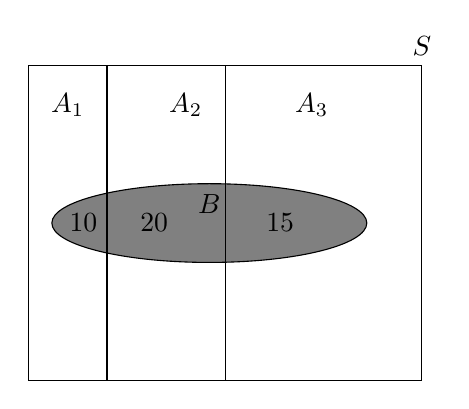
\begin{tikzpicture}[fill=gray]
		\filldraw[color=black, fill=gray] (0.3,0) ellipse (2. and 0.5) node [text=black,above] {$B$};
		\node[] at (-1.5,1.5) {$A_1$};
		\node[] at (0,1.5) {$A_2$};
		\node[] at (1.6,1.5) {$A_3$};
		\node[] at (-1.3,0) {$10$};
		\node[] at (-.4,0) {$20$};
		\node[] at (1.2,0) {$15$};
		\draw (-1.,-2) -- (-1.,2) ;
		\draw (0.5,-2) -- (0.5,2);
		\draw (-2,-2) rectangle (3,2) node[text=black,above] {$S$};
	\end{tikzpicture}
	
\end{problem} 


\begin{problem}{7} $ $
	\begin{enumerate}
		
		\item $A$ is a subset of a countable set, $\mathbb N$, and is thus countable.
		
		\item As shown in the book, if we can write any set, $S$ in the form:
		
		\begin{equation}
		S = \bigcup_{i \in \mathcal{B}} \bigcup_{j \in \mathcal C}  \{ q_{ij} \},
		\end{equation}
		where $\mathcal B$ and $\mathcal C$ are countable sets, then $S$ is a countable set.  It is easy to see that we may re-write $B$ as:
		
		\begin{equation}
		B = \bigcup_{i \in \mathbb Q} \bigcup_{j \in \mathbb Q}  \{ a_i +b_j \sqrt{2}\},
		\end{equation}
		where $q_{ij} \equiv a_i +b_j \sqrt{2}$, and thus $B$ is countable.
		
		
		\item $C$ is uncountable.  One way to prove this is to note that for all $x\in [0, 1]$, $(x, 0) \in C$, so that $C \supset [0, 1]$, i.e, $C$ is a superset of an uncountable set and is thus uncountable.
  
 	\end{enumerate}
\end{problem} 


\begin{problem}{8} I first prove that $A_n \subset A_{n+1}$ (a proper subset) for all $n=1, 2, \ldots$.  To do this, it suffices to prove that $(n-1)/n < n/(n+1)$, which I do with proof by contradiction.  By assuming $(n-1)/n \ge n/(n+1)$, after a little algebra, one concludes that $-1 \ge 0$, which is clearly a contradiction and therefore $(n-1)/n < n/(n+1)$. Thus the union of all the $A_n$s is given by the largest set in the sequence, which is $A_\infty$ ($=\lim_{n \rightarrow \infty} [0, \frac{n-1}{n})$).  After applying L'hopitals rule, one can show that $A_\infty = [0, 1)$, and thus:

	\begin{equation}
		A = \bigcup_{n=1}^{\infty} A_n = [0, 1) \nonumber .
	\end{equation}

  \end{problem} 
  
  
  \begin{problem}{9} As with the previous problem, one may show that $A_{n+1} \subset A_{n}$ for all $n=1, 2, \ldots$ by proving that $1/(n+1)<1/n$.  This is somewhat obvious, but if you really want to be formal, you can prove it with a proof by contradiction.  Therefore, the intersection of all the $A_n$s is given by the smallest set, $A_\infty$, which is $\lim_{n \rightarrow \infty} [0, \frac{1}{n}) = [0, 0) = \{ 0\}$, and thus:
	\begin{equation}
		A = \bigcap_{n=1}^{\infty} A_n = \{ 0\} \nonumber .
	\end{equation}
  \end{problem} 
  
  
    \begin{problem}{10} $ $
    \begin{enumerate}
    \item To motivate the bijection (the one-to-one mapping between $2^{\mathbb N}$ and $C$) we are about to construct, note that for every set in $2^{\mathbb N}$, a natural number $n$ will either appear once, or not at all.  Therefore, it is convenient to indicate its presence in the set with a 1 and its absence with a 0.  For example $\{1, 3, 6 \}$ will get mapped to the sequence $101001000 \ldots$ (this is implicitly assuming that we have pre-ordered the elements in the particular set from $2^{\mathbb N}$).  In general, the bijective mapping we use $f: 2^{\mathbb N} \rightarrow C$, is given by:
    \begin{equation*}
    f(x) = \mathbbm{1}(1\in x)\mathbbm{1}(2\in x) \ldots,
    \end{equation*}
    where $\mathbbm{1}$ is the so-called indicator function which is 1 if its argument evaluates to true and 0 otherwise.  To prove that this mapping is bijective, we must prove it is both injective and surjective.
 
 To prove it is injective, I use a proof by contradiction.  Assume it is not injective.  Under this assumption there exists $x, x^\prime \in 2^{\mathbb N}$, where $x\neq x^\prime$ such that $f(x) = f(x^\prime)$.  $x$ and $x^\prime$ can either have the same cardinality, or they can be different.  Without loss of generality, if they are different, let us call $x$ the one with the larger cardinality.  Since $x \neq x^\prime$ there exists at least 1 natural number $n$ in $x$ which is not in $x^\prime$.  Therefore in the sequences $f(x)$ and $f(x^\prime)$, there is at least one value in the sequences which does not match up, namely the value at position $n$, and therefore $f(x) \neq f(x^\prime)$, which violates our original assumption.
 
 The proof of surjectivity is also straightforward.
     
     \item Any number in $x \in [0, 1)$ always has a unique binary expansion given by $x = b_1/2+b_2/2^2+...$, and therefore we can construct a bijective mapping between $x \in [0, 1)$ and $C$ by computing $b_1/2+b_2/2^2+...$, and then by dropping the 0. at the beginning of the sequence.  Since there is a bijection between $2^{\mathbb N}$ and $C$ and a bijection between $C$ and $[0, 1)$ (and given the fact that the composition of 2 bijections is a bijection) there is thus a bijection between $2^{\mathbb N}$ and $[0, 1)$.  Assuming (correctly so) that the interval $[0, 1)$ is uncountable, then so too is $2^{\mathbb N}$.
     
     
     
     \end{enumerate}
     
  \end{problem} 
  
  
    \begin{problem}{11} $ $
 As shown in the previous problem, there is a bijection between $[0, 1)$ and $C$.  Therefore, if $C$ is uncountable, then so too is $[0, 1)$.  We can use what is known as Cantor's diagonal argument to prove that $C$ is uncountable.
 
 Let us try to search for a bijective mapping between $C$ and $\mathbb N$.  Suppose, for example, that the first few mappings are given by:
 \\

 \begin{tabular}{ c c c }
1 & $\rightarrow$ & $\mathbf{0} 000000\ldots$ \\
2 & $\rightarrow$& $1\mathbf{1}11111\ldots$\\
3 & $\rightarrow$& $01 \mathbf{0}1010\ldots$\\
4& $\rightarrow$ &$101\mathbf{0}101\ldots$\\
5 & $\rightarrow$&$1101\mathbf{0}11\ldots$\\
6& $\rightarrow$&$00110\mathbf{1}1\ldots$\\
7 &$\rightarrow$& $100010\mathbf{0}\ldots$ \\
& $\vdots$&  
 \end{tabular}


Let us now construct a new sequence, $s \in C$ by enumerating the complement of the elements along the diagonal of the mapping (which I have highlighted in boldface above), $s = 1011101 \ldots$.  By construction, $s$ differs from every proposed mapping since the $n^{th}$ digit in $s$ is different than the $n^{th}$ digits in all of the mappings.   Thus, no natural number gets mapped to $s$, and hence the proposed mapping is not surjective.  The mappings I chose for illustration in this example for $1, \ldots, 7$ were arbitrary, and this argument applies to any potential mapping.  Therefore, there is no bijective mapping between $\mathbb N$ and $C$, and hence no bijection between $[0, 1)$ and $\mathbb N$.  Thus, the interval $[0, 1)$ is uncountable.
 
 
  \end{problem}
  
\begin{problem}{12} $ $
	\begin{enumerate}
		
		\item The domain is $\{ H, T \}^3$ and the codomain is $\mathbb N \cup \{ 0 \}$
		
		\item $range(f) = \{0, 1, 2, 3\}$
		
		\item $x$ can be all triplets that contain exactly 2 heads: $(H, H, T)$, $(H, T, H)$ or $(T, H, H)$.
  
 	\end{enumerate}
\end{problem} 


\begin{problem}{13} $ $
	\begin{enumerate}
		
		\item The universal set is partitioned by the events $a$, $b$, $d$, and thus $P(b) = 1 - P(a) - P(d) = 1-0.5-0.25=0.25$.
		
		\item Since the events $b$ and $d$ are disjoint, by the 3rd axiom of probability, $P(b \cup d) = P(b)+P(d) = 0.25+0.25 = 0.5 $.
	
  
 	\end{enumerate}
\end{problem} 


\begin{problem}{14} $ $
	\begin{enumerate}
		
		\item By inclusion-exclusion: $P(A \cap B) = P(A)+P(B)-P(A \cup B) = 0.4+0.7-0.9 = 0.2$.
		
		\item 
			\begin{align*}
				P(A^c \cap B) &= P(B-A) \\
				& = P(B) - P(A\cap B) \\
				& = 0.7-0.2 \\
				&=0.5
			\end{align*}
			
		\item 
			\begin{align*}
				P(A-B) & = P(A) - P(A\cap B) \\
				& = 0.4-0.2 \\
				&=0.2
			\end{align*}
			
		\item  By drawing the Venn diagram, one can see that
			\begin{align*}
				P(A^c-B) & = P(S) - P(A\cup B) \\
				& = 1 - 0.9 \\
				&=0.1,
			\end{align*}
		where $S$ is the universal set.
		
		
		\item  By drawing the Venn diagram, one can see that
			\begin{align*}
				P(A^c \cup B) & = P(S) - P(A- B) \\
				& = 1 - 0.2 \\
				&=0.8.
			\end{align*}

		\item  
			\begin{align*}
				P(A \cap (B \cup A^c)) &=  P((A \cap B)\cup(A \cap A^c) )\\
				& = P((A \cap B) \cup \emptyset)\\
				&= P(A \cap B) \\
				& = 0.2.
			\end{align*}
  
 	\end{enumerate}
\end{problem} 



  \begin{problem}{15} $ $
	\begin{enumerate}
		
		\item The second roll is independent of the first, so we only need to consider the second roll, in which case $P(X_2 = 4) = 1/6$ since this is a finite sample space with equal probabilities for all outcomes.
		
	\item The sample space is $\{1, 2, \ldots, 6 \} \times \{1, 2, \ldots, 6 \}$, which has a cardinality of 36, and the possible outcomes corresponding to the event that $X_1 +X_2 = 7$ are given by the set \\
	$\{ (1, 6), (6, 1), (2, 5), (5, 2), (3, 4), (4, 3) \}$, which has a cardinality of 6, and therefore $P(X_1+X_2 = 7) = 6/36=1/6$.
		
		\item Listing out the tuples that satisfy the second condition in a matrix-like representation, we have: 
		
			\begin{equation*}
				\begin{array}{ccc}
					(1, 4) & (1, 5)& (1, 6) \\
					(2, 4) & (2, 5)& (2, 6) \\
 					& \vdots & \\
					(6, 4) & (6, 5) & (6, 6) \\
				\end{array},
			\end{equation*}
of which there are $3\times 6$ elements.  However, the first condition does not allow the elements $(2, 4)$, $(2, 5)$, $(2, 6)$, and thus the total size of the event space is  $3\times 6-3 =15$.  Thus $P(X_1 \ne 2 \cap X_2 \ge 4) = 15/36=5/12$.
	
  
 	\end{enumerate}
\end{problem} 


\begin{problem}{16} $ $
	\begin{enumerate}
		
		\item The formula for a geometric series will be useful here: $\sum_{k=0}^{\infty} c r^k = a/(1-r)$ for $|r|<1$.  To solve for $c$, we can use the normalization constraint:
		
		\begin{align*}
			1 &= \sum_{k=1}^{\infty} P(k) \\
			& = -c+\sum_{k=0}^{\infty} c\left (\frac{1}{3} \right)^k \\
			& = -c +\frac{c}{1-1/3}, 
		\end{align*}
and therefore $c=2$.

		\item 
			\begin{align*}
			P(\{ 2, 4, 6\}) &=P(\{2 \} \cup \{ 4 \} \cup \{6\}) \\
			& = P(2)+P(4)+P(6) \\
			& =2\left[\frac{1}{3^2}+ \frac{1}{3^4}+\frac{1}{3^6}\right] \\
			& = \frac{182}{729}
			\end{align*}
			
		\item 
			\begin{align*}
			P(\{ 3, 4, 5, \ldots \}) &= 2\sum_{k=3}^{\infty} \left( \frac{1}{3}\right)^k \\
			&= -2\left[1+\frac{1}{3} +\frac{1}{9} \right]+ 2\sum_{k=0}^{\infty} \left( \frac{1}{3}\right)^k \\
			& = - 2 \left( \frac{13}{9} \right) +2\left(\frac{3}{2}\right) \\
			& =\frac{1}{9}
			\end{align*}
  This answer may also have been computed $1-P(1)-P(2)$.
 	\end{enumerate}
\end{problem} 



\begin{problem}{17} Let us write down what we know in equations.  Let $a$, $b$, $c$, $d$ represent the events that teams, A, B, C and D win the tournament respectively.  Then as stated in the problem, $P(a) = P(b)$, $P(c)=2P(d)$ and $P(a \cup c)=0.6$.  Since the events partition the sample space, $P(a \cup c)=P(a)+P(c)$.  We know one more equation, which is that the probabilities must sum to one: $P(a)+P(b)+P(c)+P(d)=1$.  We therefore have a linear system with 4 equations and 4 unknowns, and it will thus be convenient to write this in matrix notation in order to solve for the probabilities:

	\begin{equation*}
		  \begin{bmatrix}
			1 &-1&0&0\\
			0&0&1&-2 \\
			1&0&1&0 \\
			1&1&1&1
		  \end{bmatrix}
 		 \begin{bmatrix}
			P(a)\\
			P(b)\\
			P(c)\\
			P(d)
		  \end{bmatrix}
		  =
		  \begin{bmatrix}
			0 \\
			0 \\
			0.6 \\
			1
		  \end{bmatrix}.
	\end{equation*}
	
$\implies$
	
	\begin{align*}
 		 \begin{bmatrix}
			P(a)\\
			P(b)\\
			P(c)\\
			P(d)
		  \end{bmatrix}
		  & =
		  \begin{bmatrix}
			1 &-1&0&0\\
			0&0&1&-2 \\
			1&0&1&0 \\
			1&1&1&1
		  \end{bmatrix}^{-1}
		  \begin{bmatrix}
			0 \\
			0 \\
			0.6 \\
			1
		  \end{bmatrix} \\
		  & =  \begin{bmatrix}
			2 &1&-3&2\\
			1&1&-3&2 \\
			-2&-1&4&2 \\
			-1&-1&2&-1
		  \end{bmatrix}
		  \begin{bmatrix}
			0 \\
			0 \\
			0.6 \\
			1
		  \end{bmatrix}\\
		  &=
		  \begin{bmatrix}
			0.2 \\
			0.2 \\
			0.4 \\
			0.2
		  \end{bmatrix}.
	\end{align*}
Notice that, as required, the probabilities sum to 1.

\end{problem} 

\begin{problem}{18} $ $
	\begin{enumerate}
		\item $P(T \le 1) = \frac{1}{16}$
		
		\item 
			\begin{align*}
				P(T>2) &= 1 - P(T\le 2) \\
				&= 1-\frac{4}{16} \\
				&=\frac{3}{4}
			\end{align*}
			
		\item
			\begin{align*}
				P(1\le T \le 3) &= P(T \le 3) - P(T < 1) \\
				&= \frac{9}{16}-\frac{1}{16} \\
				&=\frac{1}{2}
			\end{align*}
			
  
 	\end{enumerate}
\end{problem} 

\begin{problem}{19} The solutions to the quadratic are given by the quadratic formula:

	\begin{equation}
		X = \frac{-1 \pm \sqrt{1-4AB}}{2A},
	\end{equation}
	which has real solutions iff the condition $1-4AB \ge 0$ is satisfied.  We therefore seek the probability that $P(1-4AB\ge 0)$ (in the unit square), which, since the point $(A, B)$ is picked uniformly, is the fraction of area in the unit square which satisfies this constraint.  Therefore points which satisfy the following inequalities contribute to this probability:

	\begin{equation*}
		\frac{1}{4} \left(\frac{1}{x} \right)\ge y,
	\end{equation*}
	
	\begin{equation*}
		x\le1
	\end{equation*}
	and
		\begin{equation*}
		y\le1,
	\end{equation*}
where the last 2 inequalities follow since the randomly drawn points must lie within the unit square.  The area in the unit square which satisfies these constraints is shown in Fig.~\ref{fig:prob_19}.


	\begin{figure}[t]
	\centering
      		 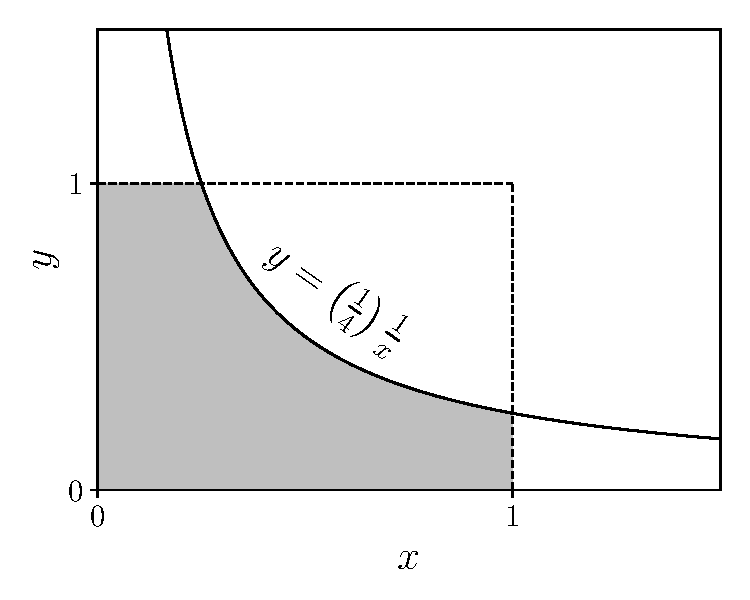
\includegraphics[totalheight=6cm]{chpt1/prob19.pdf}
  			  \caption{area of unit square resulting in real solutions}
    			   \label{fig:prob_19}
	\end{figure}
It is clear from the figure that the area is given by:

\begin{align*}
	P(\mathrm{real~solns.}) & = \frac{1}{4} +\frac{1}{4}\int_{1/4}^1\frac{1}{x} dx \\
	& = \frac{1}{4}+\frac{1}{4} \ln 4 \\
	& \approx 0.60.
\end{align*}
	
\end{problem} 


\begin{problem}{20} $ $

\begin{enumerate}
\item To solve this problem, note that:
	\begin{equation*}
		A\equiv \bigcup_{i=1}^{\infty}A_i = A_1 \cup (A_2-A_1) \cup (A_3-A_2) \cup \ldots, 
	\end{equation*}
where in the figure, $A_1$ is the innermost circle, $(A_2-A_1)$ is the ``annulus" around $A1$, $(A_3-A_2)$ is the next ``annulus" and so-forth.  It is clear that the union of $A_1$ and all of the annuli results in $A$, and that each of these regions are also disjoint.  I utilize the previous equation in the desired proof:
	\begin{figure}[t]
	\centering
      		 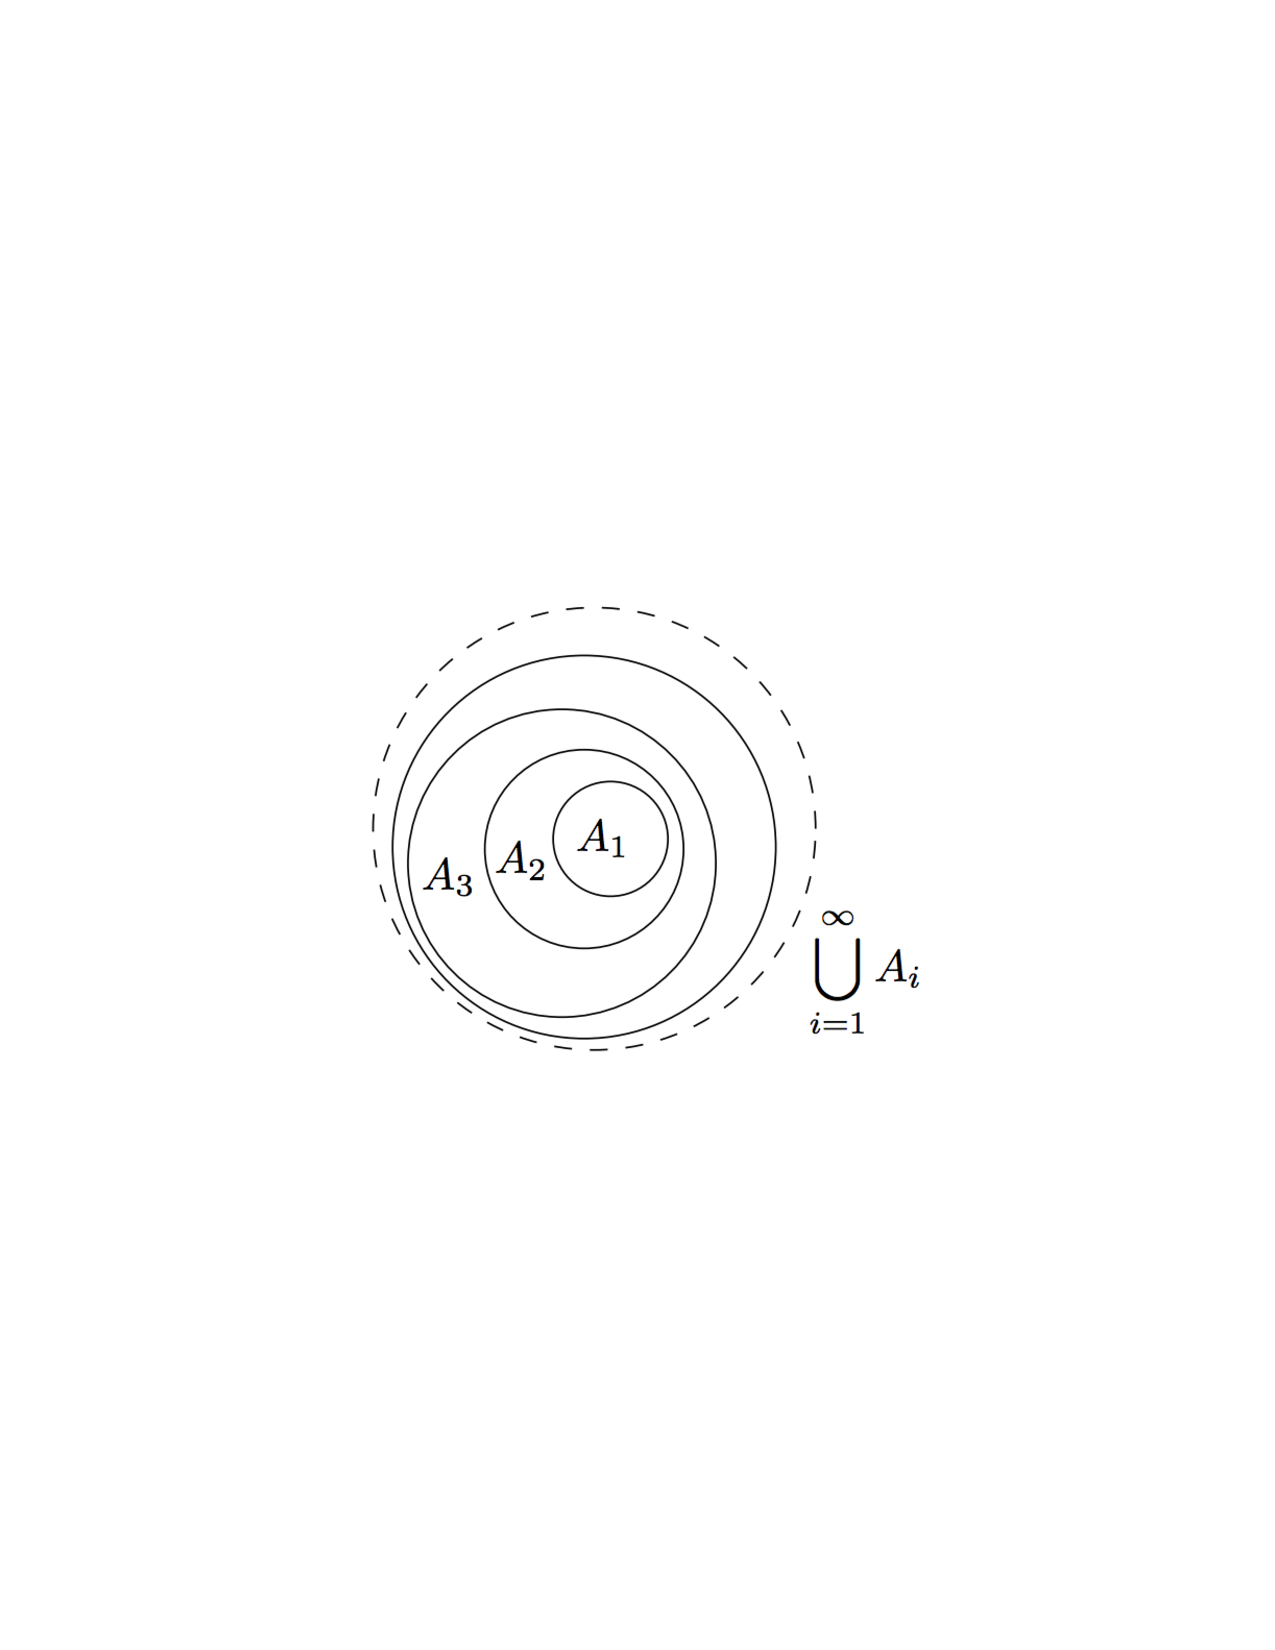
\includegraphics[totalheight=6cm]{chpt1/prob20.pdf}
  			  \caption{Venn diagram of events $A_1, A_2, \ldots$}
    			   \label{fig:prob_20}
	\end{figure}
	
	\begin{proof}
		\begin{align*}
		P(A) & = P(A_1)+\sum_{i=2}^{\infty} P(A_i-A_{i-1}) \\
		& = P(A_1)+\lim_{n \rightarrow \infty} \sum_{i=2}^{n} P(A_i-A_{i-1}) \\
		& = P(A_1)+\lim_{n \rightarrow \infty} \sum_{i=2}^{n} \left [P(A_i)-P(A_{i-1}) \right] \\
		& =  P(A_1)+\lim_{n \rightarrow \infty} \{ [P(A_2)-P(A_1)]+[P(A_3)-P(A_2)]+[P(A_4)-P(A_3)] \\
		& +\ldots +[P(A_n)-P(A_{n-1})]\} \\
		& = P(A_1)+\lim_{n \rightarrow \infty} [P(A_n)-P(A_1)] \\
		& = \lim_{n \rightarrow \infty} P(A_n) \qedhere
		\end{align*}
	\end{proof}
	
	\item Redefining $A$: $A\equiv \bigcap_{i=1}^{\infty}A_i$, we seek to find $P(A)$. If $A_1, A_2, \ldots$ is a series of decreasing events, then $A_1^c, A_2^c, \ldots$ must be a series of increasing events, and we can can therefore utilize the results of the part (a) on sequence of the complements (as well as De Morgan):
	
	\begin{align*}
		P(A^c) = P\left(\left(\bigcap_{i=1}^{\infty}A_i\right)^c\right)=P\left(\bigcup_{i=1}^{\infty}A_i^c\right) = \lim_{n \rightarrow \infty}P(A_n^c).
	\end{align*}
	
	A few more steps completes the proof:
	
		\begin{proof}
		\begin{align*}
		P(A) & = 1-P(A^c) \\
		& = 1 - \lim_{n \rightarrow \infty}P(A_n^c) \\
		& = \lim_{n \rightarrow \infty} [1 - P(A_n^c)]\\
		 & = \lim_{n \rightarrow \infty} P(A_n) \qedhere
		\end{align*}
	\end{proof}
	
	
\end{enumerate}
	
\end{problem} 

\begin{problem}{21} $ $
	\begin{enumerate}
		\item
			Let us define new events, $B_i$, such that $B_1$ =$A_1$, $B_2 =A_2-A_1$, $B_3= A_3-A_2-A_1, \ldots$.  Note that the $B_i$s are disjoint.  Also note that:
			
			\begin{align*}
			\bigcup_{i=1}^n B_i & = A_1 \cup (A_2-A_1) \cup (A_3-A_2-A_1) \cup \ldots  \cup (A_n-A_{n-1}-\ldots -A_1)\\
			&=A_1\cup A_2 \cup A_3 \ldots \cup A_n\\
			&=\bigcup_{i=1}^n A_i,
			\end{align*}
and for the same reason $\bigcup_{i=1}^\infty B_i=\bigcup_{i=1}^\infty A_i$.  Using these facts, the proof is now straightforward:

		\begin{proof}
		\begin{align*}
		P\left(\bigcup_{i=1}^\infty A_i \right) &= P\left(\bigcup_{i=1}^\infty B_i\right) \\
		& = \sum_{i=1}^\infty P(B_i) \\
		& = \lim_{n \rightarrow \infty} \sum_{i=1}^n P(B_i) \\
		& = \lim_{n \rightarrow \infty} P\left (\bigcup_{i=1}^n B_i \right) \\
		& = \lim_{n \rightarrow \infty} P\left (\bigcup_{i=1}^n A_i \right)  \qedhere
		\end{align*}
	\end{proof}
	
	\item The prove this second result I use the previous result as well as De Morgan (twice):
	
		\begin{proof}
		\begin{align*}
		P\left (\bigcap_{i=1}^\infty A_i \right) &= P\left( \bigcup_{i=1}^\infty A_i^c \right) \\
		& = \lim_{n \rightarrow \infty} P\left(\bigcup_{i=1}^n A_i^c \right) \\
		& =\lim_{n \rightarrow \infty} P\left(\bigcap_{i=1}^n A_i\right)  \qedhere
		\end{align*}
	\end{proof}
			
	\end{enumerate}

\end{problem} 


\begin{problem}{22} Let $A_{coff}$ be the event that a customer purchases coffee and $A_{cake}$ be the event that a customer purchases cake.  We know that $P(A_{coff}) = 0.7$, $P(A_{cake}) = 0.4$ and $P(A_{coff}, A_{cake}) = 0.2$.  Thus, the conditional probability we seek is:

	\begin{equation*}
		P(A_{coff}|A_{cake}) = \frac{P(A_{coff}, A_{cake})}{P(A_{cake}) } = \frac{0.2}{0.4}=0.5.
	\end{equation*}

\end{problem} 

\begin{problem}{23} $ $
	\begin{enumerate}
		\item 
			\begin{equation*}
				P(A|B) = \frac{P(A \cap B)}{P(B)} = \frac{0.1+0.1}{0.1+0.1+0.1+0.05} \approx 0.57
			\end{equation*}
			
		\item 
			\begin{equation*}
				P(C|B) = \frac{P(C \cap B)}{P(B)} = \frac{0.1+0.05}{0.1+0.1+0.1+0.05} \approx 0.43
			\end{equation*}
			
		\item 
			\begin{equation*}
				P(B|A \cup C) = \frac{P(B\cap ( A\cup C))}{P( A\cup C)} = \frac{0.1+0.1+0.05}{0.1+0.2+0.1+0.1+0.05+0.15} \approx 0.36
			\end{equation*}
			
		\item 
			\begin{equation*}
				P(B|A, C) = \frac{P(B \cap (A \cap C))}{P(A \cap C)} = \frac{0.1}{0.1+0.1} =0.5
			\end{equation*}
		
	\end{enumerate}

\end{problem} 



\begin{problem}{24} $ $
	\begin{enumerate}
		\item 
			\begin{equation*}
				P(2 \le X \le 5) = \frac{3}{10} =0.3
			\end{equation*}
			
		\item 
			\begin{equation*}
				P(X \le 2| X \le 5) = \frac{2}{5} =0.4
			\end{equation*}
		
		\item 
			\begin{equation*}
				P(3 \le X \le 8| X \ge 4) = \frac{P(3 \le X \le 8 \cap X \ge 4)}{P(X \ge 4)} = \frac{4}{6} = \frac{2}{3}
			\end{equation*}		
		
	\end{enumerate}

\end{problem} 


\begin{problem}{25} Let $ON$ denote the event that a student lives on campus, $OFF$ denote the event that a student lives off campus and $A$ denote the event that a student receives an A.  Given the data I compute the following probabilities:

\begin{equation*}
P(ON) \approx \frac{200}{600} =\frac{1}{3}
\end{equation*}

\begin{equation*}
P(A) \approx \frac{120}{600} =\frac{1}{5}
\end{equation*}

\begin{equation*}
P(A \cap ON) = P(A) - P(A \cap OFF) \approx \frac{1}{5} - \frac{80}{600} = \frac{1}{15}
\end{equation*}

If the events $ON$ and $A$ are independent, then $P(A \cap ON)  = P(A)P(ON)$.  Looking at the probabilities above, we see that the data suggests this relationship, and thus the data suggests that getting an A and living on campus are independent. 

\end{problem} 


\begin{problem}{26}  Let $N_1$ be the number of times out of $n$ that a 1 is rolled, $N_6$ be the number of times out of $n$ that a 6 is rolled and $X_i$ be the value of the $i^{th}$ roll.  Then:

\begin{align*}
	P(N_1 \ge 1 \cap N_6 \ge 1) &= 1 - P((N_1 \ge 1 \cap N_6 \ge 1)^c) \\
	&= 1 - P(N_1= 0 \cup N_6=0) \\
	& = 1-[P(X_1 \ne 1, X_2 \ne 1, \ldots, X_n \ne 1)+P(X_1 \ne 6, X_2 \ne 6, \ldots, X_n \ne 6) \\
	& - P((X_1 \ne 1, X_2 \ne 1, \ldots, X_n \ne 1)\cap (X_1 \ne 6, X_2 \ne 6, \ldots, X_n \ne 6))] \\
	& =1-\left [ \left (\frac{5}{6} \right )^n+\left (\frac{5}{6}\right)^n - P(X_1 \ne 1, X_1 \ne 6, X_2 \ne 1, X_2 \ne 6, \ldots, X_n \ne 1 X_n \ne 6)\right] \\
	& =1-\left [2 \left (\frac{5}{6} \right )^n - P(X_1 \ne 1, X_1 \ne 6)^n \right] \\
	& = 1-\left [ 2\left (\frac{5}{6} \right )^n-\left (\frac{4}{6} \right )^n \right] \\
	& =1 - \frac{2(5^n) -4^n}{6^n}.
\end{align*}
In the second line I have used De Morgan, and I have also used the fact, several times, that the outcome of roll $i$ is independent of the outcome of roll $j$.  Testing for a for values of $n$, I find that, when $n=1$, the probability is 0, which makes sense because at the very minimum we would need at least one 1 and one 6, which cannot happen if we have only rolled once.  The probability then monotonically increases, which also makes sense because it becomes more and more likely that we roll at least one 1 and at least one 6 the more rolls we throw.  Note that as a sanity check, one can show that $\lim_{n \rightarrow \infty} 1 - (2(5^n) -4^n)/(6^n)$ is 1, so that our formula for the probability is bounded between 0 and 1.  Also note that this formula can also be obtained more easily with combinatorics, which will be introduced in Chapter 2.

\end{problem}

\begin{problem}{27} $ $
\begin{enumerate}
\item Refer to Fig.~\ref{fig:prob_27}
	\begin{figure}[t]
	\centering
      		 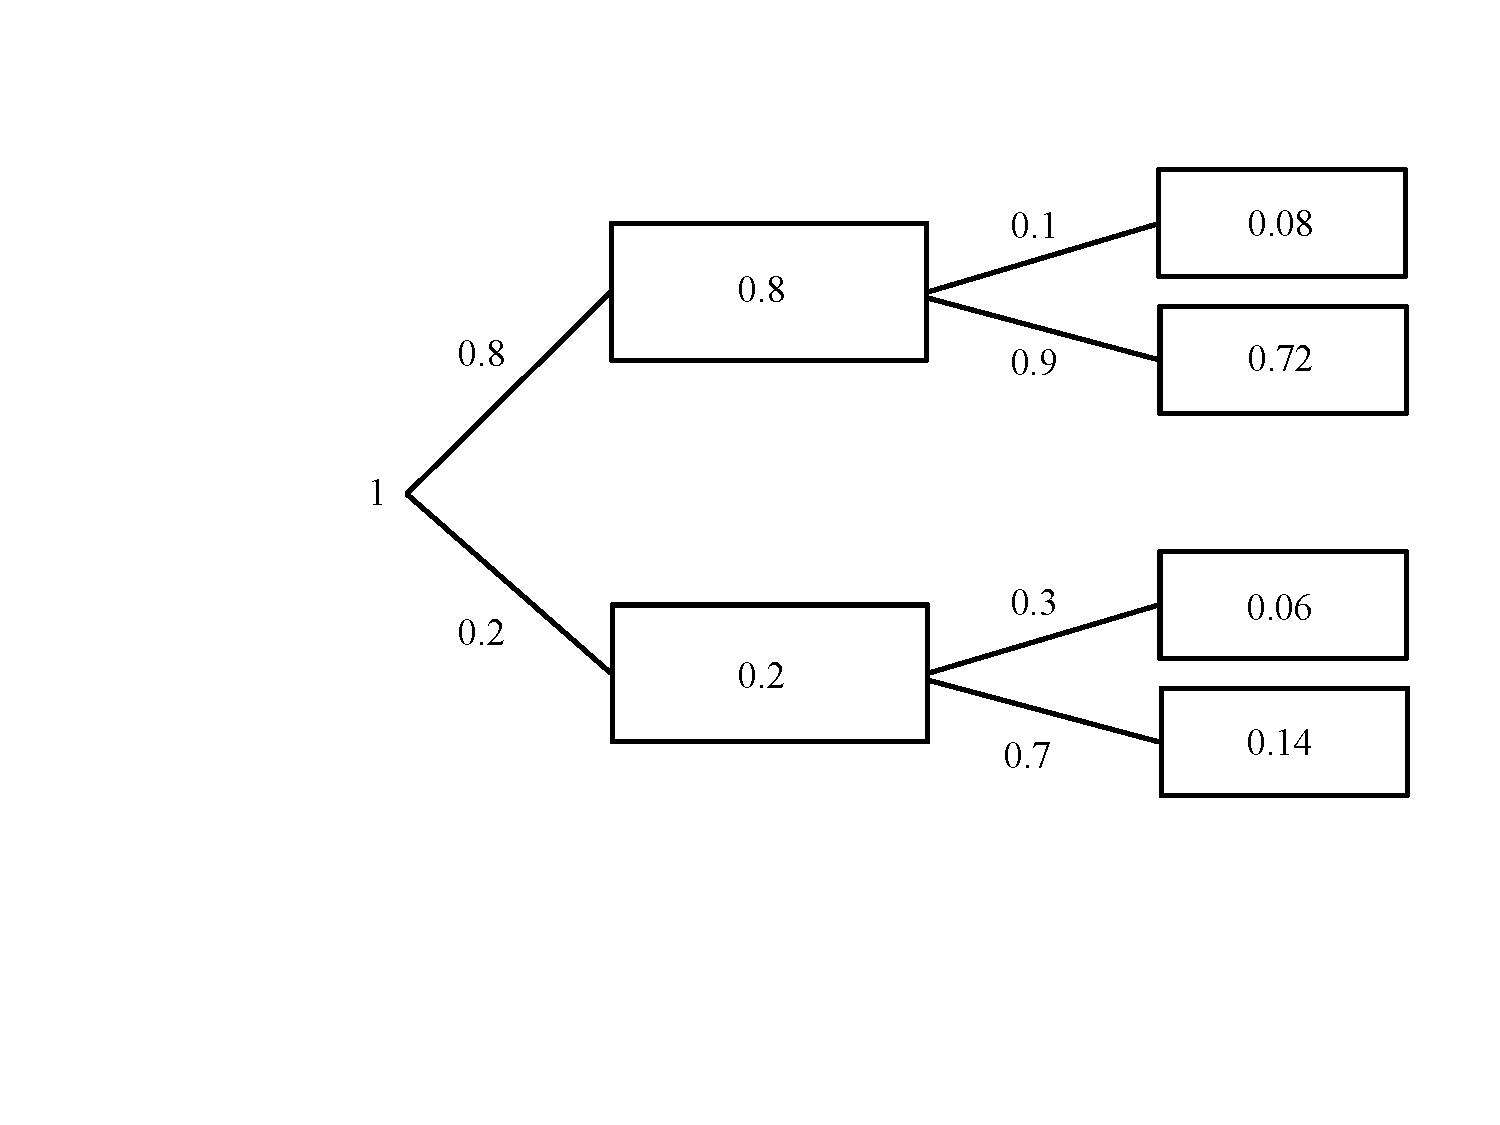
\includegraphics[totalheight=6cm]{chpt1/tree_27.pdf}
  			  \caption{Tree diagram for problem 27.}
    			   \label{fig:prob_27}
	\end{figure}
	
	\item $P(E) = P(E \cap G) + P(E \cap G^c) = 0.08+0.06=0.14$
	
	\item $P(G|E^c) = \frac{P(G \cap E^c)}{P(E^c)} =  \frac{0.72}{1-0.14} \approx 0.84$. 
	
\end{enumerate}

\end{problem}


\begin{problem}{28} Let $A_i$ be the event that the $i^{th}$ ($i=1, 2, 3$) unit of the 3 picks is defective, while the other 2 are not defective.  Note that $A_1$, $A_2$ and $A_3$ are all disjoint, since it is impossible for any unit to be both defective and not defective simultaneously.  The probability we seek is therefore:

\begin{align*}
P(A_1 \cup A_2 \cup A_3) & = P(A_1)+P(A_2)+P(A_3) \\
&= \left(\frac{5}{100}\right)\left(\frac{95}{99}\right)\left(\frac{94}{98}\right) +\left(\frac{95}{100}\right)\left(\frac{5}{99}\right)\left(\frac{94}{98}\right)+\left(\frac{95}{100}\right)\left(\frac{94}{99}\right)\left(\frac{5}{98}\right) \\
&\approx 0.14.
\end{align*}


\end{problem}




\begin{problem}{29} Let $F$ be the event that the system is functional, and $C_i$ be the event that component $i$ is functional.
	\begin{enumerate}
		\item $P(F) = P(C_1, C_2, C_3) = P_1 P_2 P_3$
		\item By inclusion-exclusion:
		\begin{align*} 
		P(F) &= P(C_1\cup C_2 \cup C_3) \\
		& = P_1+ P_2 +P_3 -P_1P_2-P_1P_3-P_2P_3+P_1P_2P_3
		\end{align*} 
		

		\item 
			\begin{align*}
				P(F) &= P((C_1, C_3) \cup (C_2, C_3)) \\
				& = P(C_1, C_3)+P(C_2, C_3) - P((C_1\cap C_3) \cap (C_2 \cap C_3)) \\
				& = P_1 P_3+P_2 P_3 - P(C_1, C_2, C_3) \\
				& = P_1 P_3+P_2 P_3 - P_1 P_2 P_3 
			\end{align*}
			
		\item $P(F) = P(C_1, C_2)+P(C_3) = P_1 P_2 +P_3 - P_1 P_2 P_3$
		\item $P(F) = P(C_1, C_2, C_5)+P(C_3, C_4, C_5) - P(C_1, C_2, C_3, C_4, C_5) = P_1 P_2 P_5+P_3 P_4 P_5 - P_1 P_2 P_3 P_4 P_5 $
	\end{enumerate}

\end{problem}
	
	
\begin{problem}{30} $ $
\begin{enumerate}
\item  The region in the unit square corresponding to set $A$ can be made more clear if we write the absolute value as a piecewise function:

\begin{equation*}
|x-y| \le \frac{1}{2} \implies
  \begin{cases}
                                   x-y \le \frac{1}{2} & \mathrm{if}~x \ge y \\
                                    y-x \le \frac{1}{2}  & \mathrm{if}~x<y \\

  \end{cases}
  \implies
  \begin{cases}
                                   y \ge - \frac{1}{2}+x & \mathrm{if}~y \le x \\
                                    y \le \frac{1}{2}+x  & \mathrm{if}~y>x \\

  \end{cases}.
\end{equation*}
This piecewise function, along with the fact that $A$ must be bounded in the unit square leads to hashed-in region in Fig.~\ref{fig:prob_30}.  The region corresponding to set $B$ is just the are in the unit square above the $45^\circ$ line (corresponding to the gray shaded region in Fig.~\ref{fig:prob_30}).

	\begin{figure}[t]
	\centering
      		 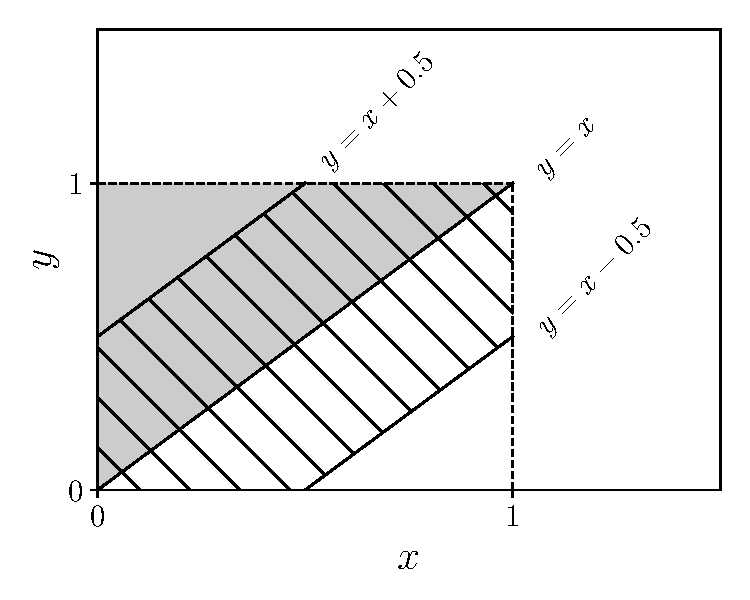
\includegraphics[totalheight=6cm]{chpt1/prob30.pdf}
  			  \caption{The unit square for Problem 30.  The shaded region represents the set $B$ and the hashed region represents the set $A$}
    			   \label{fig:prob_30}
	\end{figure}
	
\item Using a little geometry, I find: $P(A) = 1- 2\left (\frac{1}{2} \right)\left (\frac{1}{2} \right)\left (\frac{1}{2} \right) = \frac{3}{4}$ and $P(B)=\frac{1}{2}$.

\item Again, using some geometry, I find: $P(A\cap B) = \frac{1}{2} - \left (\frac{1}{2} \right)\left (\frac{1}{2} \right)\left (\frac{1}{2} \right) = \frac{3}{8}$.  Since $P(A)P(B) =  \left (\frac{3}{4} \right) \left (\frac{1}{2} \right) =\frac{3}{8}$, the 2 events are indeed independent.

\end{enumerate}

\end{problem}


\begin{problem}{31} $ $
\begin{enumerate}
\item  Let $s$ be the event that the received email is spam and $r$ be the event that the received email contains the word refinance.  From the problem statment, we know that $P(s) = 0.5$ (so that $P(s^c) = 0.5$), $P(r|s)=0.01$ and $P(r|s^c)= 0.00001$.  Using Bayes' rule:

\begin{align*}
P(s|r) &= \frac{P(r|s)P(s)}{P(r)} \\
&= \frac{P(r|s)P(s)}{P(r|s)P(s)+P(r|s^c)P(s^c)} \\
& = \frac{(0.01) (0.5)}{(0.01)(0.5)+(0.00001)(0.5)} \\
& \approx 0.999
\end{align*}

\end{enumerate}

\end{problem}

\begin{problem}{32} $ $

\begin{enumerate}

\item
There are 4 possible paths from $A$ to $B$: 1 to 4 (path 1), 2 to 5 (path 2), 1 to 3 to 5 (path 3), 2 to 3 to 4 (path 4).  Let $\mathcal P_i$ be the event that path $i$ is open.  Only 1 path needs to be open for event $A$ to occur, so the probability of $A$ is given by the probability of $\mathcal P_1$ or $\mathcal P_2$ or $\mathcal P_3$ or $\mathcal P_4$.  We expand this probability with inclusion-exclusion, making sure to enumerate all unique pairs and all unique triplets:

\begin{align*}
P(A)& = P(\mathcal P_1 \cup \mathcal P_2 \cup \mathcal P_3 \cup \mathcal P_4) \\
&= P(\mathcal P_1)+ P(\mathcal P_2)+P(\mathcal P_3)+P( \mathcal P_4) \\
&- P(\mathcal P_1\cap \mathcal P_2)-P(\mathcal P_1\cap \mathcal P_3)-P(\mathcal P_1\cap \mathcal P_4)-P(\mathcal P_2\cap \mathcal P_3)-P(\mathcal P_2\cap \mathcal P_4)-P(\mathcal P_3\cap \mathcal P_4) \\
&+P(\mathcal P_1\cap \mathcal P_2 \cap \mathcal P_3)+P(\mathcal P_1\cap \mathcal P_2 \cap \mathcal P_4)+P(\mathcal P_1\cap \mathcal P_3 \cap \mathcal P_4)+P(\mathcal P_2\cap \mathcal P_3 \cap \mathcal P_4) \\
& - P(\mathcal P_1 \cap \mathcal P_2 \cap \mathcal P_3 \cap \mathcal P_4 ) \\
&= P(B_1\cap B_4)+ P(B_2\cap B_5)+P(B_1 \cap B_3 \cap B_5)+P(B_2 \cap B_3 \cap B_4) \\
&- P((B_1\cap B_4)\cap (B_2\cap B_5))-P((B_1\cap B_4)\cap (B_1 \cap B_3 \cap B_5))-P((B_1\cap B_4)\cap (B_2 \cap B_3 \cap B_4))\\
&-P((B_2\cap B_5)\cap (B_1 \cap B_3 \cap B_5))-P((B_2\cap B_5)\cap (B_2 \cap B_3 \cap B_4))\\
&-P((B_1 \cap B_3 \cap B_5)\cap (B_2 \cap B_3 \cap B_4)) \\
&+P((B_1\cap B_4)\cap (B_2\cap B_5) \cap (B_1 \cap B_3 \cap B_5))+P((B_1\cap B_4)\cap (B_2\cap B_5) \cap (B_2 \cap B_3 \cap B_4))\\
&+P((B_1\cap B_4)\cap (B_1 \cap B_3 \cap B_5) \cap (B_2 \cap B_3 \cap B_4))\\
&+P((B_2\cap B_5)\cap (B_1 \cap B_3 \cap B_5) \cap (B_2 \cap B_3 \cap B_4)) \\
& - P((B_1\cap B_4) \cap (B_2\cap B_5) \cap (B_1 \cap B_3 \cap B_5) \cap (B_2 \cap B_3 \cap B_4) ) \\
&= P(B_1\cap B_4)+ P(B_2\cap B_5)+P(B_1 \cap B_3 \cap B_5)+P(B_2 \cap B_3 \cap B_4) \\
&- P(B_1\cap B_4\cap B_2\cap B_5)-P(B_1\cap B_4 \cap B_3 \cap B_5)-P(B_1\cap B_4\cap B_2 \cap B_3)\\
&-P(B_2\cap B_5 \cap B_1 \cap B_3 )-P(B_2\cap B_5 \cap B_3 \cap B_4)-P(B_1 \cap B_3 \cap B_5 \cap B_2 \cap B_4) \\
&+P(B_1\cap B_2 \cap B_3 \cap B_4 \cap B_5)+P(B_1\cap B_2 \cap B_3 \cap B_4 \cap B_5)\\
&+P(B_1\cap B_2 \cap B_3 \cap B_4 \cap B_5)+P(B_1\cap B_2 \cap B_3 \cap B_4 \cap B_5) \\
& - P(B_1\cap B_2 \cap B_3 \cap B_4 \cap B_5) \\
&= P_1 P_4+ P_2 P_5+P_1 P_3 P_5+P_2 P_3 P_4 - P_1 P_4 P_2 P_5-P_1 P_4 P_3 P_5-P_1 P_4 P_2 P_3\\
&-P_2 P_5 P_1 P_3 -P_2 P_5 P_3 P_4+2P_1 P_2 P_3 P_4 P_5  \\
&= P_1 P_4(1- P_2 P_5 -P_3 P_5-P_2 P_3)+ P_2 P_5+P_1 P_3 P_5+P_2 P_3 P_4 \\
&-P_2 P_5 P_1 P_3 -P_2 P_5 P_3 P_4+2P_1 P_2 P_3 P_4 P_5  \\
\end{align*}
As a sanity check, if bridge 3 does not exist (i.e., if $P_3 = 0$), then there are only 2 paths and by inclusion-exclusions, $P(A) = P_1 P_4+P_2 P_5 -P_1P_4P_2P_5$.  In the limit that $P_3=0$, we see that, indeed, the above formula matches this probability.  

\item To solve for $P(B_3|A)$ I use Bayes' rule:

\begin{equation*}
P(B_3|A) = \frac{P(A|B_3) P_3}{P(A)}.
\end{equation*}

$P(A)$ has already been calculated.  To solve for the probability of $A$ conditioned on $B_3$ we need only to condition each probability term in $P(A)$ on $B_3$, which effectively turns all the $P_3$ terms in the formula for $P(A)$ to unity.  Therefore,
\begin{equation*}
P(A|B_3) = P_1 P_4(1- P_2 P_5 -P_5-P_2)+ P_2 P_5+P_1 P_5+P_2 P_4 -P_2 P_5 P_1  -P_2 P_5 P_4+2P_1 P_2 P_4 P_5,
\end{equation*}
and we can insert $P(A|B_3)$ and $P(A)$ into Bayes' rule to obtain the answer:
\begin{align*}
&P(A|B_3) = \\
&\frac{P_1 P_4 P_3(1- P_2 P_5 -P_5-P_2)+ P_3 P_2 P_5+P_3 P_1 P_5+P_3 P_2 P_4 -P_3 P_2 P_5 P_1  -P_3 P_2 P_5 P_4+2P_1 P_2 P_3 P_4 P_5}{P_1 P_4(1- P_2 P_5 -P_3 P_5-P_2 P_3)+ P_2 P_5+P_1 P_3 P_5+P_2 P_3 P_4-P_2 P_5 P_1 P_3 -P_2 P_5 P_3 P_4+2P_1 P_2 P_3 P_4 P_5}.
\end{align*}



\end{enumerate}

\end{problem}

\begin{problem} {33}
Without loss of generality, let us call the door that you picked door 1, and let us arbitrarily denote the remaining doors by 2 and 3.  Let $C_i$ denote the event that the car is behind door $i$ and $H_i$ denote the event that the host opens door $i$.  The original probability that you guessed the door with the car is $P(C_1) = 1/3$.  Since the host will not open door 1, and he will also not open the door with the car behind it, we have the following probabilities:
\begin{align*}
&P(H_1|C_1)= 0 \\
&P(H_2|C_1)=\frac{1}{2} \\
&P(H_3|C_1)=\frac{1}{2} \\
&P(H_1|C_2) = 0 \\
&P(H_2|C_2) = 0 \\
&P(H_3|C_2) = 1 \\
&P(H_1|C_3) = 0 \\
&P(H_2|C_3) = 1 \\
&P(H_3|C_3) = 0 \\
\end{align*}
If the host opens door 3, we would like to know $P(C_2|H_3)$, because if this value is higher than 1/3, it is in our interest to switch to door 2.  Likewise if the host opens door 2, we would like to know $P(C_3|H_2)$ to know if we should switch to door 3.  Given the symmetry of the problem $P(C_2|H_3)=P(C_3|H_2)$, so I only need to compute the probability once, which I do using Baye's rule:
\begin{align*}
P(C_2|H_3) &= \frac{P(H_3|C_2)P(C_2)}{P(H_3|C_1)P(C_1)+P(H_3|C_2)P(C_2)+P(H_3|C_3)P(C_3)} \\
& = \frac{1\left(\frac{1}{3}\right)}{\left(\frac{1}{2}\right)\left(\frac{1}{3}\right)+1\left(\frac{1}{3}\right)+0} \\
& = \frac{2}{3}.
\end{align*}
It is therefore in your interest to switch to door 2 if the host opens door 3 or to switch to door 3 if the host opens door 2.





\end{problem}


\begin{problem}{34} $ $

	\begin{enumerate}
	
		\item $P(A) = 1/6$, $P(B) = |\{ (1, 6), (2, 5), (3, 4), (4, 3), (5, 2), (6, 1) \} |/36 = 1/6$, $P(A, B) = 1/36$.  Since $P(A)P(B) = 1/36 = P(A, B)$, the events are indeed independent.
		
		\item $P(C) = 1/6$, so that $P(A, C) = 1/36$, and $P(A, C) = 1/36$ and therefore they are independent.
		
		\item $P(B) P(C) = 1/36$, $P(B, C) = 1/36$, so yes, they are independent.
		
		\item The events $A$, $B$ and $A$, $C$ and $B$, $C$ are pairwise independent.  We also need to check if $P(A, B, C) =P(A)P(B)P(C)$.  The probability of $P(A, B, C)$ equals 0 since those events cannot all occur at once, whereas $P(A)P(B)P(C) \ne 0$.  Therefore, the events $A$, $B$ and $C$ are not independent.

	\end{enumerate}

\end{problem}

\begin{problem}{35} Let $X_1$ denote the outcome of the first roll, $W$ denote the event that I win, and let the probability of tails be $q$ ($=1-p$).  From Bayes', the probability that the first roll was heads is given that I won the game is:

\begin{equation*}
P(X_1 =H|W) = \frac{P(W|X_1 =H) P(X_1 =H)}{P(W)}.
\end{equation*}
I first calculate the probability of winning:

\begin{align*}
P(W) &= P(HH)+P(THH)+P(HTHH)+P(THTHH) + \ldots \\
& = P(HH)+P(HTHH)+ \ldots+P(THH)+P(THTHH)+ \ldots \\
&= q^0p^2+qp^3+\ldots +qp^2+q^2p^3 +\ldots \\
& = (q^0p+qp^2+\ldots)p +(q^0 p^2+q p^3 +\ldots)q 
\end{align*}

Note that since $P(W) = P(W|X_1=H)p+P(W|X_1=T)q$, the first term in the parentheses in the above equation represents $P(W|X_1=H)$ while the second term in the parentheses represents $P(W|X_1=T)$.  I solve for both of these seperately:

\begin{align*}
P(W|X_1=H) &= q^0p+qp^2+\ldots \\
&= (qp)^0 p+ (qp)^1 p+\ldots \\
& = p\sum_{k=0}^\infty{(qp)^k} \\
&=\frac{p}{1-qp},
\end{align*}
while
\begin{align*}
P(W|X_1=T) &= q^0 p^2+q p^3 +\ldots \\
&= (qp)^0 p^2+ (qp)^1 p^2+\ldots \\
& = p^2\sum_{k=0}^\infty{(qp)^k} \\
&=\frac{p^2}{1-qp},
\end{align*}
where I have used the formula for a geometric series.  Thus we can compute the probability of winning as 
\begin{align*}
P(W) &= P(W|X_1=H)p+P(W|X_1=T)q \\
& = \frac{p^2}{1-qp}+\frac{p^2q}{1-qp}
\end{align*}

Finally, we can plug all of these formulas into Bayes' equation:

\begin{align*}
P(X_1 =H|W) &= \frac{P(W|X_1 =H) P(X_1 =H)}{P(W)} \\
& =\frac{ \frac{p^2}{1-qp}}{\frac{p^2}{1-qp}+\frac{p^2q}{1-qp}} \\
& = \frac{1}{1+q} \\
& = \frac{1}{2-p}.
\end{align*}

\end{problem}

\begin{problem}{36}  Let $H_{n+1}$ denote the event that the $(n+1)^{th}$ flip is a head, $H \ldots H$ denote the event of observing $n$ heads and $F$ denote the event that we pick the fair coin.  We would like to find $P(H_{n+1}|H \ldots H)$, and we know that from the law of total probability $P(H_{n+1}) = P(H_{n+1}|F)P(F)+P(H_{n+1}|F^c)P(F^c)$.  By conditioning all of the probabilities on $H \ldots H$, this equation gives a formula for the probability we desire:

\begin{equation}
P(H_{n+1}|H \ldots H) = P(H_{n+1}|F, H \ldots H)P(F|H \ldots H)+P(H_{n+1}|F^c, H \ldots H)P(F^c|H \ldots H).
\end{equation}

The terms  $P(H_{n+1}|F, H \ldots H)$ and $P(H_{n+1}|F^c, H \ldots H)$ are conditionally independent of $H \ldots H$ given $F$ (or $F^c$) and therefore these probabilities are 1/2 and 1 respectively.  We may obtain $P(F|H \ldots H)$ from Bayes' rule:

\begin{align*}
P(F|H \ldots H) &= \frac{P(H \ldots H|F)P(F)}{P(H \ldots H|F)P(F)+P(H \ldots H|F^c)P(F^c)} \\
& = \frac{\left (\frac{1}{2}\right)^n \frac{1}{2}}{\left (\frac{1}{2}\right)^n \frac{1}{2}+\frac{1}{2}} \\
& \frac{1}{1+2^n}.
\end{align*}

Thus:

\begin{align*}
P(H_{n+1}|H \ldots H) &= \left (\frac{1}{2} \right)\frac{1}{1+2^n}+\left (1-\frac{1}{1+2^n} \right) \\
& = 1-\frac{1}{2(1+2^n)}.
\end{align*}

We can check this formula for the extremes that $n=0$ and $n \rightarrow \infty$.  In the first case, if $n=0$, we can calculate the probability of heads directly: $P(H) = (1/2)(1/2)+1(1/2) = 3/4$, which matches what the formula predicts when $n=0$.  When $n \rightarrow \infty$, we would expect that the coin is probably unfair, so that the probability of the next flip landing heads is 1.  Indeed, this is what the formula predicts in the limit that $n \rightarrow \infty$.

\end{problem}



\begin{problem} {37} Let $X_i$ denote the number of girls for the $i^{th}$ child.  Note that $X_i$ can only take on values 0 or 1.  We seek the probability $P(X_{1} =1, \ldots, X_{n} =1|X_1+ \ldots +X_n \ge 1)$.  This can be re-written with Bayes' rule:

\begin{equation}
P(X_{1} =1, \ldots, X_{n} =1|X_1+ \ldots +X_n \ge 1)= \frac{P(X_1+ \ldots +X_n \ge 1|X_{1} =1, \ldots, X_{n} =1)P(X_1=1, \ldots, X_n=1)}{P(X_1+ \ldots +X_n \ge 1)}.
\end{equation}

In the numerator, the first term is just 1 since $X_1+\ldots +X_n$ is guaranteed to be at least 1 if all $X_1, \ldots, X_n$ are equal to 1.  The second term is $(1/2)^n$ since all boy/girl events are independent.  To calculate the denominator, it is easier to consider its complement: $P(X_1+ \ldots +X_n \ge 1) = 1 - P(X_1+ \ldots +X_n=0)=1-P(X_1=0, \ldots, X_n=0)=1-(1/2)^n$.  Putting all of these into Bayes' rule, I obtain:


\begin{equation*}
P(X_{1} =1, \ldots, X_{n} =1|X_1+ \ldots +X_n \ge 1)= \frac{1}{2^n-1}.
\end{equation*}

We can test this formula for low values of $n$.  For $n=1$, $P(X_1=1|X_1=1) =1$, which the above formula predicts.  For $n=2$, by listing out the boy/girl event space,  it is not difficult to determine that $P(X_1=1, X_2=1| X_1+X_2\ge1) = 1/3$, which also what the above formula predicts.

\end{problem}

\begin{problem}{38} Let $L$ be the event that the family has at least 1 daughter named Lilia, $G\ldots G$ be the event that the $n$ children are girls, $BG\ldots G$ be the event that the first child is a boy and the following $n-1$ children are girls, $GBG\ldots G$ be the event that the first child is a girl, the second is a boy and following $n-2$ children are girls, etc....  We are interested in $P(G\ldots G|L)$ which we can obtain with Bayes' rule:

\begin{equation}
P(G\ldots G|L) = \frac{P(L|G\ldots G) P(G\ldots G)}{P(L)}.
\end{equation}
The denominator is given by:
\begin{align*}
P(L) &= 1- P(L^c) \\
&=1-P(G\ldots G)[P(L^c|G\ldots G)+P(L^c|BG\ldots G)+P(L^c|GBG\ldots G)+ \ldots +P(L^c|B \ldots B)] \\
&=1-P(G\ldots G)[(1-\alpha)^n+(1-\alpha)^{n-1}+(1-\alpha)^{n-1}+\ldots + (1-\alpha)^0] \\
&=1-P(G\ldots G)\sum_{k=0}^n \frac{n!}{k!(n-k!)}(1-\alpha)^k \\
&=1-P(G\ldots G)(2-\alpha)^n.
\end{align*}
In the third line I used the fact that to have no daughters named Lilia given $n$ daughters, the daughters need to be not be named Lilia $n$ times, which occurs with probability $(1-\alpha)^n$.  In the fourth line, I used the fact that the total number of sequences of $BG\ldots G$, $GBG\ldots G$, ..., is given by the number of permutations of $n$ elements ($n!$) divided by the number of repeats for any element (which for the $G$s is $k!$, where $k$ is the number of $G$s in the sequence, and which for the $B$s is $(n-k)!$).  This is a simple combinatorics problem which will be discussed in the following chapter.  Finally, to solve the summation, I used the binomial theorem.

We need one more probability, which is $P(L|G\ldots G) = 1 - P(L^c|G\ldots G) = 1 - (1-\alpha)^n$.  Sticking in all of these probabilities into Baye's rule, I obtain:

\begin{align*}
P(G\ldots G|L)& = \frac{[1 - (1-\alpha)^n]\left (\frac{1}{2}\right)^n}{1-\left (\frac{1}{2}\right)^n(2-\alpha)^n} \\
& = \frac{1-(1-\alpha)^n}{2^n-(2-\alpha)^n} \\
& \approx \frac{1-(1-n\alpha)}{2^n-2^n(1-\frac{n\alpha}{2})} \\
& = \frac{1}{2^{n-1}},
\end{align*}
where I have used a Taylor expansion to simplify the polynomial terms since $\alpha \ll 1$. The case of $n=2$ corresponds to Problem 7 of section 1.4.5 in the book.  Evaluating my formula with $n=2$ I find that $P(GG|L) = (2-\alpha)/(4-\alpha)\approx 1/2$ which is the same formula as the answer to Problem 7 of section 1.4.5.

\end{problem}


\begin{problem}{39} Let $R$ be the event that a randomly chosen child is a girl, and $G\ldots G$ be the event that the family has $n$ girls.  We seek to find $P(G\ldots G|R)$, which we can get from Bayes' rule:

\begin{equation*}
P(G\ldots G|R) = \frac{P(R|G\ldots G) P(G\ldots G) }{P(R)}.
\end{equation*}
$R$ is certain to happen conditioned on $G\ldots G$, $P(G\ldots G)$ is simply $(1/2)^n$ and the probability of randomly choosing a girl from a family without any prior information about genders is 1/2 as shown for the $n=1$ ($S=\{G,  B\}$) and $n=2$ ($S=\{BB, BG, GB, GG\}$) cases below:

$n=1:$
\begin{equation*}
P(R) = P(R|G)P(G)+P(R|B)P(B) = 1\left (\frac{1}{2}\right)+0\left(\frac{1}{2}\right) = \frac{1}{2},
\end{equation*}

$n=2:$
\begin{align*}
P(R) &= P(R|BB)P(BB)+P(R|BG)P(BG) +P(R|GB)P(GB)+P(R|GG)P(GG) \\
&= 0\left (\frac{1}{4}\right)+\left (\frac{1}{2}\right)\left (\frac{1}{4}\right) +\left (\frac{1}{2}\right)\left (\frac{1}{4}\right) +1\left (\frac{1}{4}\right) \\
&= \frac{1}{2}.
\end{align*}
Therefore $P(G\ldots G|R) = 1/2^{n-1}$.



\end{problem}










  

